\chapter{Applicazione per il personale Information Technology}\label{sec:2App}
In questo capitolo si descrive la seconda applicazione sviluppata presentando i requisiti, la progettazione, lo sviluppo e i test.\\
\\L'applicazione per il personale del gruppo information technology (IT) ha lo scopo di registrare le attività giornaliere effettuate dai dipendenti.IT
Si è realizzata anche una \glossario{dashboard} che facilita i dirigenti nella valutazione delle migliori strategie, bilanciamento ed organizzazione del lavoro. 
E' importante analizzare principalmente l’ultimo periodo e non tutto lo storico delle attività registrate perchè lo scopo è valutare il lavoro e i prodotti ottenuti decidendo per il futuro prossimo se apportare alcune modifiche strategiche all'organizzazione e bilanciamento del tempo lavorativo.\\
Per sviluppare questa applicazione sono stati utilizzati i seguenti strumenti, descritti nel capitolo dedicato alle tecnologie:
\begin{itemize}
    \item Microsoft List;
    \item Power Apps;
    \item Power BI;
    \item Power Automate.
\end{itemize}
\newpage%%%%%%%

\section{Analisi dei Requisiti}\label{sec:2App-Requisiti}
\renewcommand{\arraystretch}{1.5} %aumento ampiezza righe
I requisiti dell'applicazione per il personale dell'information technology sono presentati e classificati nella \tablename \space \ref*{tab:Requisiti-IT}. 
\begin{table}[H]
  \begin{tabular}{ |m{6em}|m{28em}| }
    \hline
    \textbf{Codice} & \textbf{Descrizione requisito} \\
    \hline
    \textbf{RFO01-IT} & Inserimento dell’attività specificando per quale organizzazione \\
    \hline
    \textbf{RFO02-IT} & Divieto di inserimento anticipato di attività future \\
    \hline
    \textbf{RFO03-IT} & Modifica ed eliminazione solo delle proprie attività \\
    \hline
    \textbf{RFO04-IT} & Eliminazione automatica degli inserimenti di oltre un anno prima \\
    \hline
    \textbf{RFD05-IT} & Filtri nella visualizzazione grafica dei dati \\
    \hline
    \textbf{RVO01-IT} & Applicazione sviluppata in ambiente Microsoft \\
    \hline
    \textbf{RVO02-IT} & La raccolta dei dati tramite \glossario{Microsoft Lists} \\
    \hline
    \textbf{RVO03-IT} & Visualizzazione grafica dei dati in \glossario{Power Bi} \\
    \hline
    \textbf{RQD01-IT} & Schermata home di benvenuto nell’applicazione \\
    \hline
    \textbf{RQF02-IT} & Filtri per agevolare la ricerca delle proprie attività inserite \\
    \hline
  \end{tabular}
\caption{Classificazione requisiti dell'applicazione dati del magazzino}
\label{tab:Requisiti-IT}
\end{table}

\section{Progettazione}\label{sec:2App-Progettazione}
Le attività svolte dai dipendenti degli uffici vengono raccolte tramite un form compilabile sull'applicazione sviluppata in \glossario{Power Apps}.
Inoltre nell'applicazione si visualizzano tutte le proprie attività registrate con la possibilità di poterle modificare o cancellare.\\ 
Ogni attività registrata viene salvata in una lista di \glossario{Microsoft Lists} collocata nel sito \glossario{SharePoint} dei dipendenti. 
La lista deve essere necessariamente salvata in un sito online, è sufficiente nella \glossario{intranet} aziendale, affinchè sia visibile ed utilizzabile dai servizi di \glossario{PowerPlatform}.\\
Lo scopo principale è di monitorare la produttività dell’ultimo periodo quindi si è stabilito di prevedere l’eliminazione automatica delle attività dopo un anno tramite un flusso \glossario{Power Automate}.\\
Per facilitare l’analisi della produttività e una visione a colpo d’occhio si è progettata una \glossario{dashboard} interattiva con \glossario{Power BI} che selezionando le singole voci permette di vedere, direttamente nel grafico, le relative distribuzioni per tipologia.\\
La seguente \figurename \space \ref*{fig:IT-Schema} illustra schematicamente l'idea di progettazione con le relative tecnologie.
\begin{figure}[H]
  \centering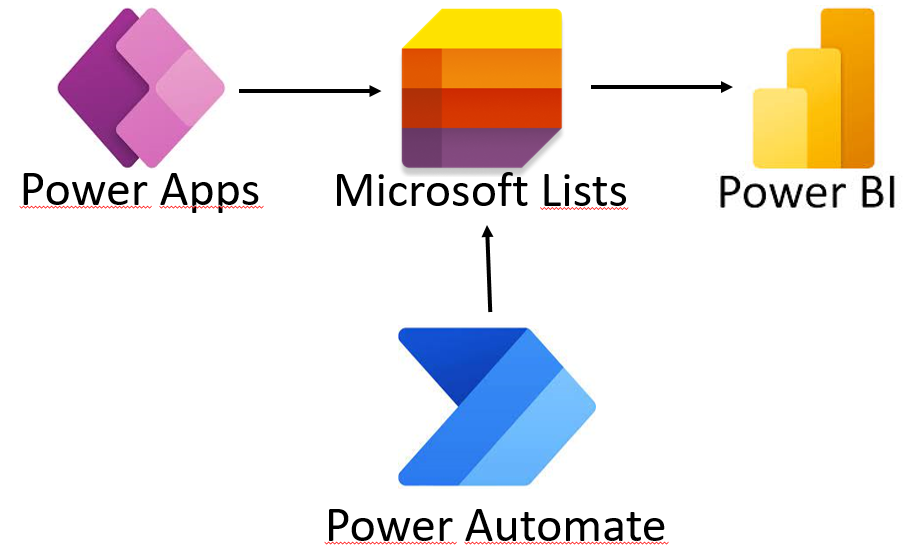
\includegraphics[width=0.8\textwidth, height=0.8\textheight,keepaspectratio]{immagini/IT-schema.png}
  \caption{Schema delle tecnologie dell'applicazione per il personale IT}
  \label{fig:IT-Schema}
\end{figure}

\section{Sviluppo}\label{sec:2App-Sviluppo}
\subsection{Microsoft Lists}
Lo sviluppo è iniziato con l'aggiunta di una nuova lista all'interno del sito creato mediante la piattaforma \glossario{SharePoint}, il cui accesso è riservato ai dipendenti dell'ufficio information technology. 
La lista è stata creata mediante \glossario{Microsoft Lists} inserendo le seguenti colonne con le relative impostazioni:
\begin{itemize}
  \item \textbf{Created By:} colonna testuale a riempimento automatico che memorizza il nome dell'utente che sta inserendo il nuovo \glossario{record};
  \item \textbf{Project:} colonna testuale in cui si può scrivere il titolo / progetto a cui si sta lavorando;
  \item \textbf{Organization:} colonna con elenco a scelta (group, location, division) in cui specificare per quale organizzazione aziendale si sta lavorando, la compilazione è obbligatoria;
  \item \textbf{Activity:} colonna con elenco a scelta (meetings, service desk, training, \dots) in cui specificare quale attività si sta svolgendo, la compilazione è obbligatoria;
  \item \textbf{Date:} colonna di tipo data in cui inserire la data di svolgimento, la compilazione è obbligatoria; 
  \item \textbf{Hours:} colonna numerica in cui inserire le ore dedicate, la compilazione è obbligatoria;
  \item \textbf{Note:} colonna testuale in cui si possono scrivere note aggiuntive.
\end{itemize}
Creata la lista che funge da database di salvataggio informazioni, \figurename \space \ref*{fig:IT-Lista} con \glossario{record} di attività  già inserite,  si è proceduto con lo sviluppo dell'applicazione mediante \glossario{Power Apps}.\\
\begin{figure}[ht]
  \centering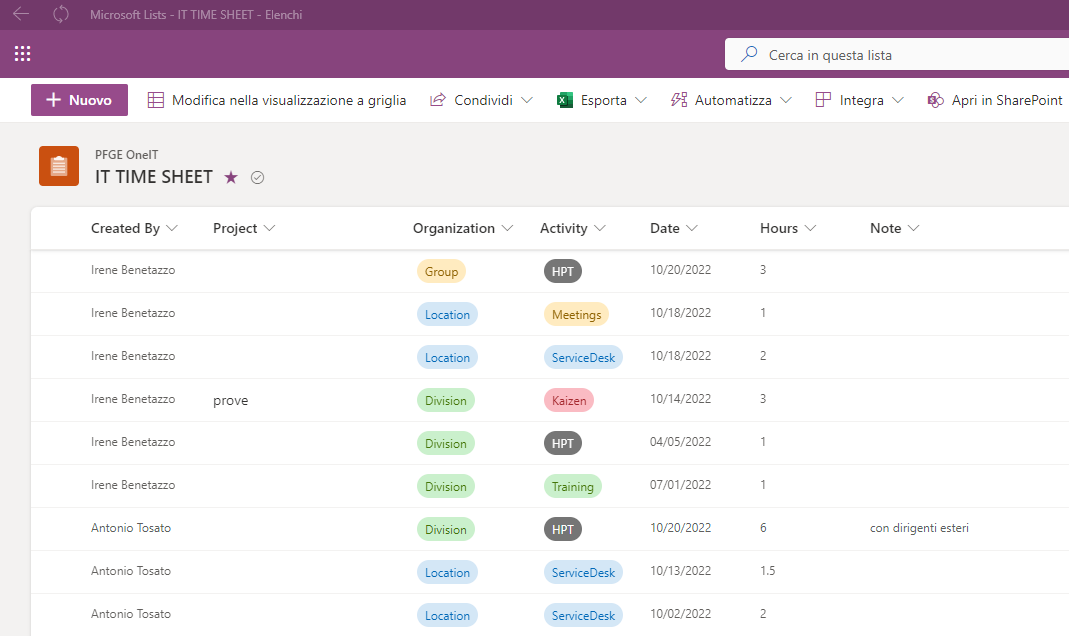
\includegraphics[width=1\textwidth, height=1\textheight,keepaspectratio]{immagini/IT-lista.png}
  \caption{Lista attività IT in Microsoft Lists}
  \label{fig:IT-Lista}
\end{figure}
\newpage %%%%%%%
\subsection{Power Apps}
La prima schermata è di benvenuto, \figurename \space \ref*{fig:IT-Home}, con due pulsanti per scegliere e collegati alla rispettiva schermata successiva.
\begin{figure}[H]
  \centering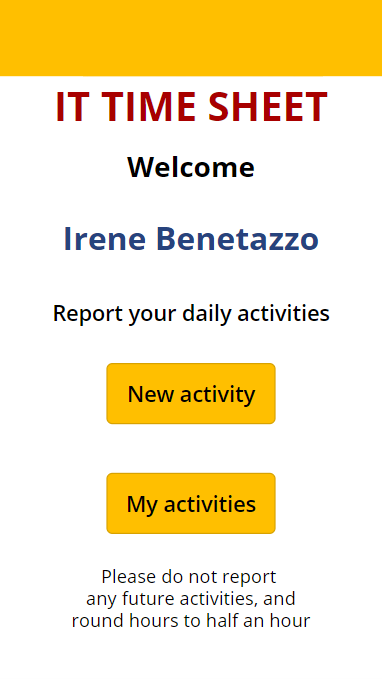
\includegraphics[width=0.5\textwidth, height=0.5\textheight,keepaspectratio]{immagini/IT-home.png}
  \caption{Schermata home dell'applicazione IT}
  \label{fig:IT-Home}
\end{figure}
Per la registrazione di una nuova attività si apre una schermata con un nuovo form da compilare collegato direttamente alla lista, in fase di sviluppo dell'applicazione si può solo scegliere di quali campi visualizzare o modificare il contenuto ma non è possibile aggiungere nuovi campi.
In caso ci sia qualche errore nella compilazione del form, esempio si lascia vuoto un campo obbligatorio, viene visualizzato un messaggio di errore.
In fase di sviluppo è stato aggiunto anche il controllo sulla data inserita che non sia una data futuristica visto lo scopo di registrare le attività svolte e non la previsione di esse.\\
Il pulsante "Save" invia il form compilato generando un nuovo \glossario{record} nella lista e riporta l'utente alla schermata di benvenuto.
La \figurename \space \ref*{fig:IT-New} mostra questa schermata.\\
\begin{figure}[H]
  \centering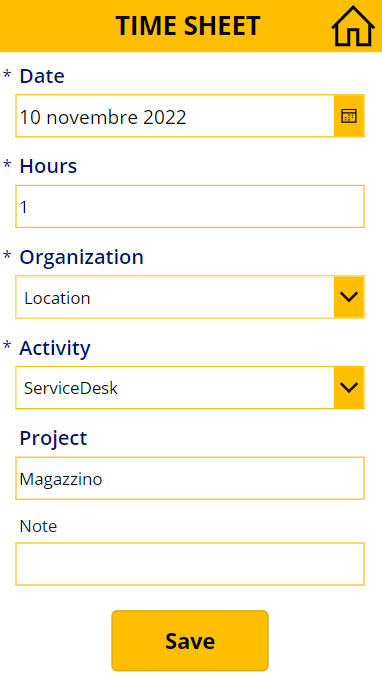
\includegraphics[width=0.5\textwidth, height=0.5\textheight,keepaspectratio]{immagini/IT-new.png}
  \caption{Schermata per la registrazione di una nuova attività o modifica}
  \label{fig:IT-New}
\end{figure}
In un'altra schermata dell'applicazione si possono visualizzare le proprie attività registrate, si offre la possibilità di filtrare l'elenco per periodo, organizzazione e attività; quindi è stata impostata la seguente formula per la visualizzazione dell'elenco:\\
\texttt{SortByColumns(Filter([@'IT TIME SHEET'];\\'Created By'.DisplayName=User().FullName \\
\&\& (Date>=DateFrom.SelectedDate \&\& Date<=DateTo.SelectedDate)\\|| (IsBlank(DateFrom) \&\& IsBlank(DateTo))\\
\&\& (Organization.Value=OrganizationChoose.Selected.Value\\|| OrganizationChoose.Selected.Value=Blank())\\ 
\&\& (Activity.Value=ActivityChoose.Selected.Value\\|| ActivityChoose.Selected.Value=Blank()));"Date";Descending)}\\
\textit{L'unica parte non chiara di questo codice potrebbe essere la parte finale del codice <<"Date";Descending>> in quanto completa le specifiche dell'istruzione iniziale di ordinamento degli elementi per data in ordine discendente.}\\
Il pulsante "Reset" pulisce i filtri ottenendo nuovamente l'elenco completo delle proprie registrazioni di attività.\\ 
Se si seleziona un'attività la si può modificare venendo rimandati alla schermata della nuova attività ma con il form già compilato, ciò è possibile grazie all'uso di una variabile nascosta che indica in quale modalità si è senza creare un ulteriore schermata per l'applicazione.
Inoltre c'è il pulsante per eliminare l'attività registrata, l'eliminazione è definitiva ed immediata anche sulla lista; infine è presente il pulsante che permette di annullare la selezione.
Da questa schermata non è mai automatico il ritorno all'homepage ma solo tramite l'icona home in alto a destra.
La \figurename \space \ref*{fig:IT-View} mostra questa schermata.\\
\begin{figure}[H]
  \centering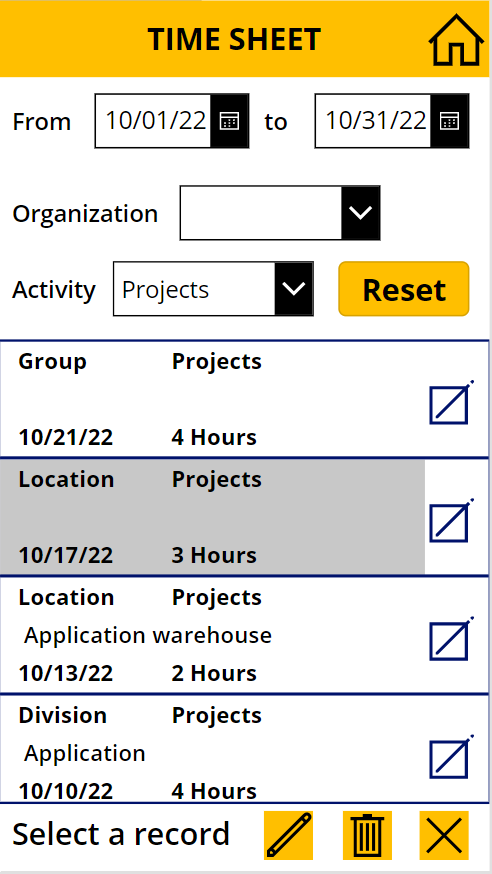
\includegraphics[width=0.5\textwidth, height=0.5\textheight,keepaspectratio]{immagini/IT-view.png}
  \caption{Schermata per la visualizzazione delle proprie attività registrate}
  \label{fig:IT-View}
\end{figure}
\newpage %%%%%%%
\subsection{Power Automate}
Per soddisfare il requisito dell'eliminazione automatica delle attività registrate si è utilizzato \glossario{Power Automate} sviluppando un flusso di istruzioni che automaticamente una volta al mese elimina le attività registrate più di un anno prima.
Al fine di non perdere le storiche registrazioni vengono salvate su una nuova lista a parte che non è collegata a nient'altro ma funge solo da registro storico.\\
La \figurename \space \ref*{fig:IT-PowerAutomate} illustra questa procedura, lo sviluppo di essa consisteva nel scegliere quale azione eseguire impostandone i relativi parametri ed accessi.
\begin{figure}[H]
  \centering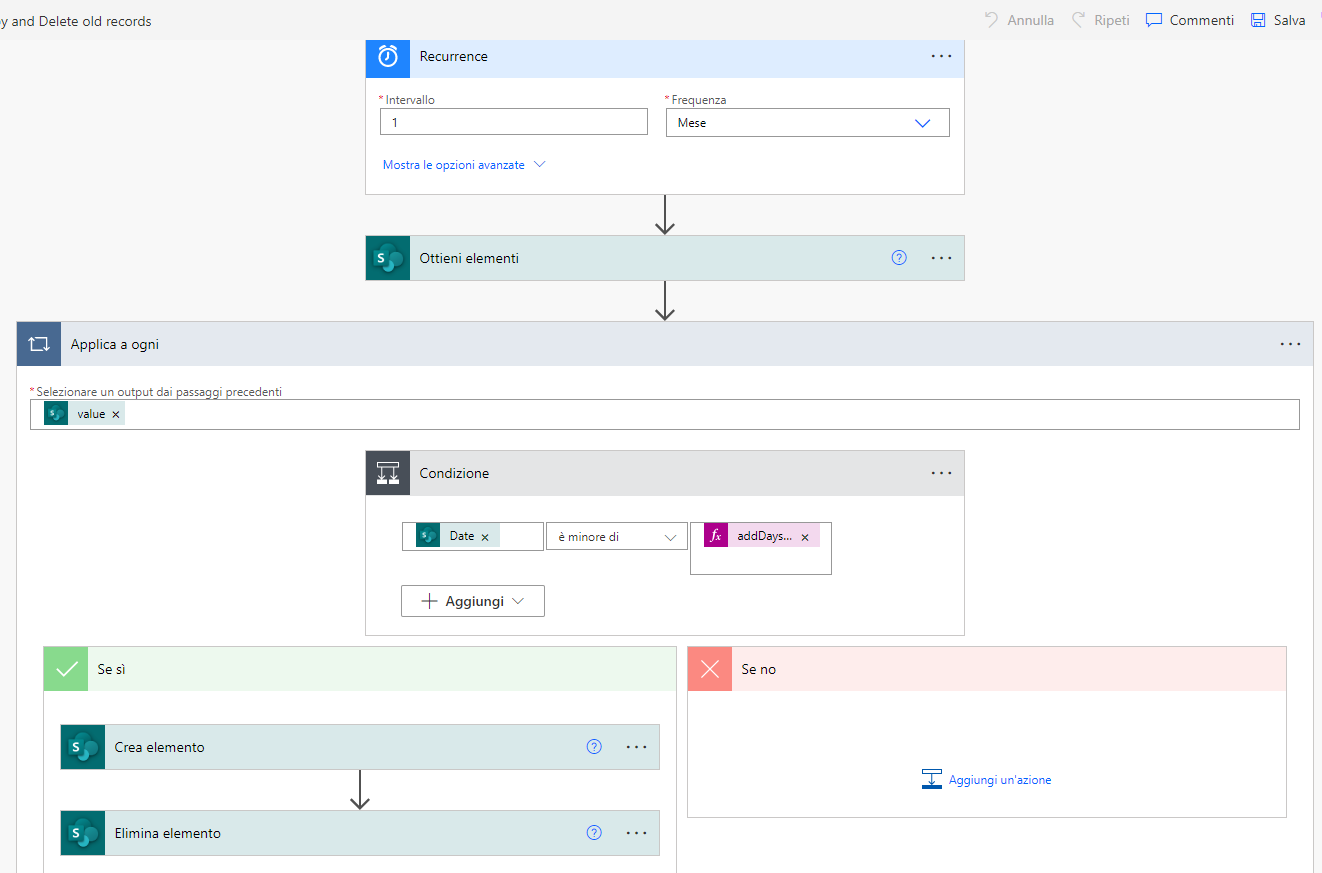
\includegraphics[width=1\textwidth, height=1\textheight,keepaspectratio]{immagini/IT-PowerAutomate.png}
  \caption{Procedura di Power Automate per la pulizia della lista IT}
  \label{fig:IT-PowerAutomate}
\end{figure}
\subsection{Power BI}
Lo sviluppo di un report grafico utilizzando il software \glossario{Power BI} versione desktop, inizia caricando i collegamenti alle liste e tabelle dei database che si vuole visualizzare.
Le tabelle caricate si possono modificare eliminando colonne non utili ai fini grafici, si può aggiungere una nuova colonna scrivendo manualmente la formula in linguaggio \glossario{DAX} o determinando il contenuto del campo in base al valore di un'altra colonna della stessa riga, ad esempio è stato fatto ciò per avere i mesi testuali, \figurename \space \ref*{fig:IT-PowerBImonth}.\\
Inoltre viene offerta la possibilità di creare nuove tabelle tramite il linguaggio \glossario{DAX} o di usufruire tra le loro proposte come il calendario.
\begin{figure}[H]
  \centering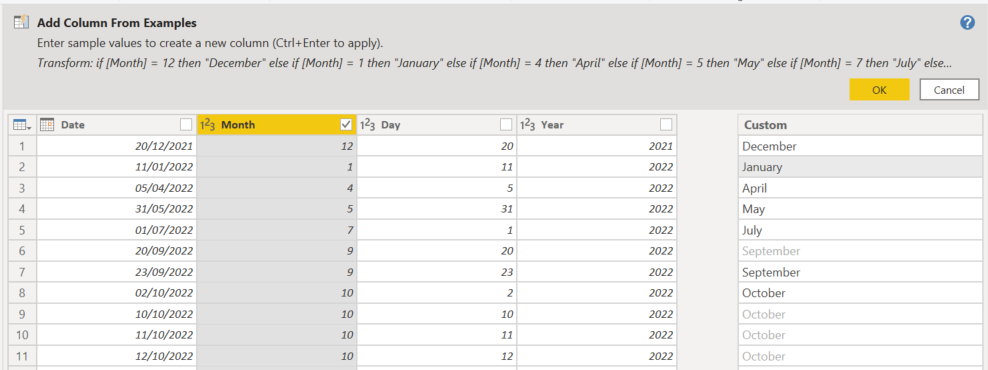
\includegraphics[width=1\textwidth, height=1\textheight,keepaspectratio]{immagini/IT-PowerBI_MonthText.png}
  \caption{Power BI aggiunta colonna personalizzata}
  \label{fig:IT-PowerBImonth}
\end{figure}
Le tabelle importate e create vengono messe in relazione tra loro specificando i campi e il tipo di relazione cioè se uno a uno o se uno a molti, in \figurename \space \ref*{fig:IT-PowerBIrelazione} si illustrano le tabelle e le relative colonne coinvolte in questo report per l'analisi delle attività dei dipendenti dell'information technology.\\
\begin{figure}[H]
  \centering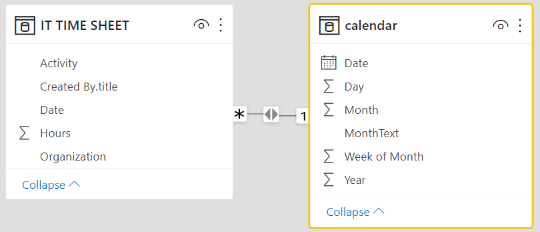
\includegraphics[width=0.8\textwidth, height=0.8\textheight,keepaspectratio]{immagini/IT-PowerBI_relazione.png}
  \caption{Power BI relazione tabelle}
  \label{fig:IT-PowerBIrelazione}
\end{figure}
Successivamente si passa allo sviluppo grafico della \glossario{dashboard}, il software mette a disposizione molti tipi di grafici e non solo tra cui scegliere.
Si è optato per i grafici a torta con suddivisione in base alla tipologia di attività e grafici ad istogrammi con le colonne composte da colori diversi per evidenziare anche la suddivisione di tipologia oltre al totale mensile.
In alto a destra è presente un riquadro che mostra il totale delle ore.\\
Di default il software offre la scheda filtri a lato della visualizzazione del report ma si possono aggiungere filtri personalizzati direttamente nella singola schermata di visualizzazione del report.
Con la selezione dei filtri si ottiene la visualizzazione solo di quei dati a schermo, mentre volendo focalizzarsi su un solo aspetto si può cliccare la voce interessata direttamente sul grafico comportando cambi di tonalità dei colori anche negli altri grafici al fine di mostrare come quel dato è distribuito.\\
La \figurename \space \ref*{fig:IT-PowerBIdashboard} mostra la \glossario{dashboard} sviluppata per questo prodotto con qualche filtro e la focalizzazione sull'attività di tipo "Projects", i riquadri neri arrotondati intorno ai grafici sono stati aggiunti per una questione puramente estestica.
\begin{figure}[H]
  \centering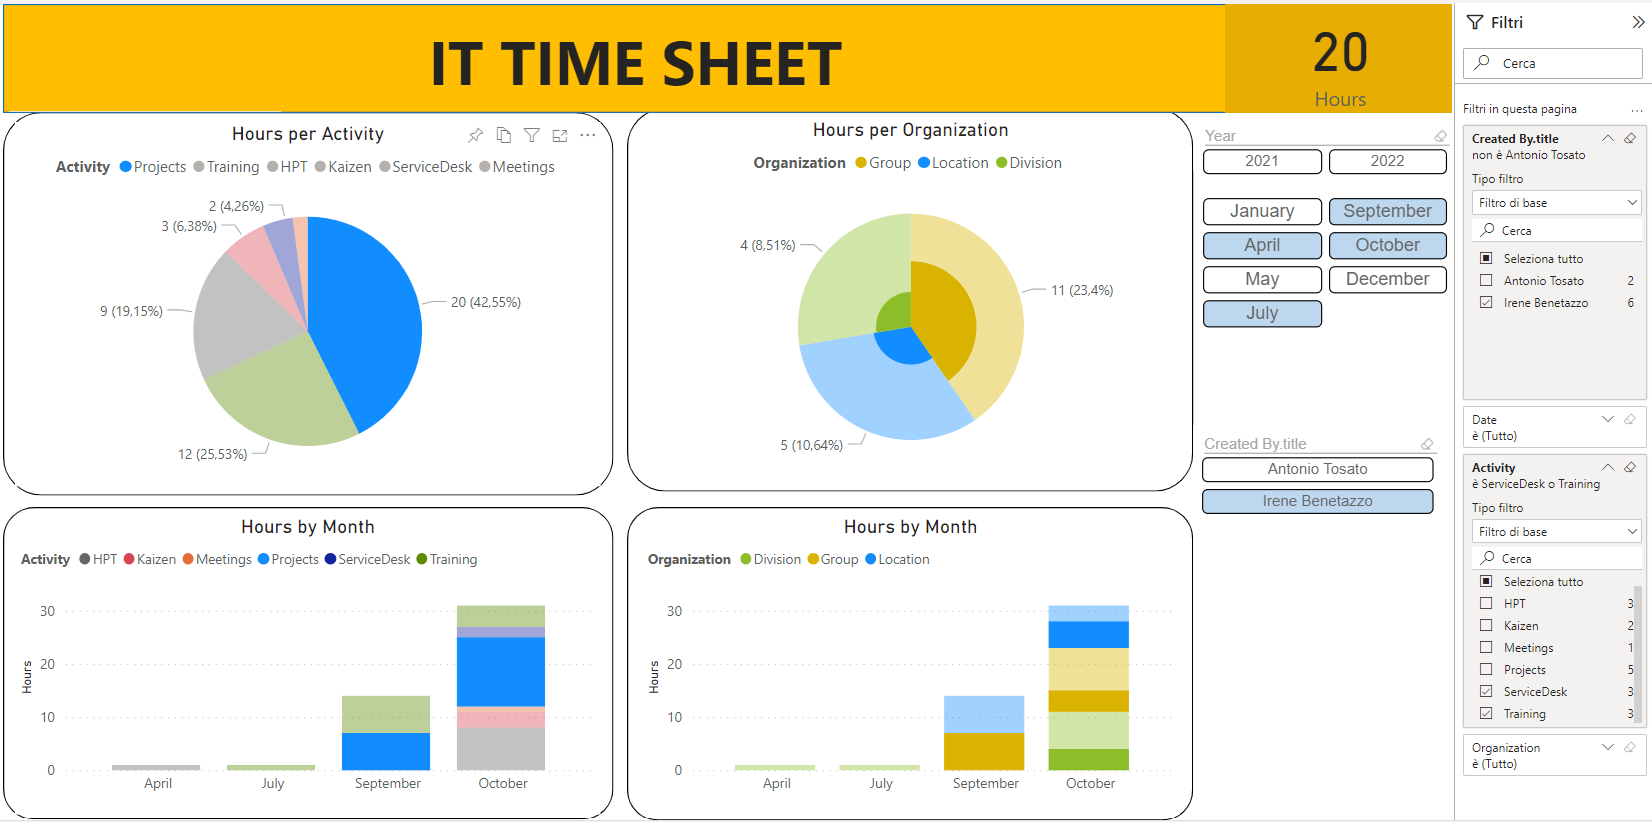
\includegraphics[width=1\textwidth, height=1\textheight,keepaspectratio]{immagini/IT-PowerBI_dashboard.png}
  \caption{Power BI dashboard IT}
  \label{fig:IT-PowerBIdashboard}
\end{figure}

\section{Verifica e Validazione}\label{sec:2App-Verifica}
Per la verifica essendo l'applicazione e la \glossario{dashboard} sviluppate mediante software basati sul principio low-code risulta difficile effettuare i classici test.
Si è quindi svolta una minimale analisi statica cioè rilettura delle formule e impostazioni inserite per configurare gli elementi.
Principalmente si è effettuata analisi dinamica facendo girare l'applicazione e la \glossario{dashboard} eseguendo test d'uso anche di casi estremi così da vederne eventuali bug o comportamenti imprevisti.\\
Durante l'analisi si è rilevato che il report in \glossario{Power BI} non si aggiornava automaticamente all'inserimento di un nuovo record nella lista. 
La soluzione è stata creare un nuovo flusso di istruzioni mediante \glossario{Power Automate} che prevede il refresh automatico dei dati nel report ogni minuto.\\
La validazione è stata effettuata insieme al tutor aziendale che ha controllato il funzionamento del prodotto in tutte le sue parti e il soddisfacimento dei requisiti stilati che viene riportato nella seguente \tablename \space \ref{tab:RequisitiSoddisfatti-IT}, i codici corrispondono alla descrizione nella tabella \ref{tab:Requisiti-IT}.
\renewcommand{\arraystretch}{1.5} %ampiezza righe
\begin{table}[H]
\begin{center}
  \begin{tabular}{ |m{6em}|m{6em}| }
    \hline
    \textbf{Codice} & \textbf{Stato} \\
    \hline
    \textbf{RFO01-IT} & Soddisfatto \\
    \hline
    \textbf{RFO02-IT} & Soddisfatto \\
    \hline
    \textbf{RFO03-IT} & Soddisfatto \\
    \hline
    \textbf{RFO04-IT} & Soddisfatto \\
    \hline
    \textbf{RFD05-IT} & Soddisfatto \\
    \hline
    \textbf{RVO01-IT} & Soddisfatto \\
    \hline
    \textbf{RVO02-IT} & Soddisfatto \\
    \hline
    \textbf{RVO03-IT} & Soddisfatto \\
    \hline
    \textbf{RQD01-IT} & Soddisfatto \\
    \hline
    \textbf{RQF02-IT} & Soddisfatto \\
    \hline
  \end{tabular}
  \caption{Classificazione requisiti dell'applicazione IT}
  \label{tab:RequisitiSoddisfatti-IT}
\end{center}
\end{table}